
\documentclass[12pt]{extarticle}
\usepackage[utf8]{inputenc}
%\usepackage{cite}
\usepackage[autolang=other,backend=biber,dateabbrev=false,sorting=none]{biblatex}
\usepackage{graphicx}
\usepackage{pdfpages}

\addbibresource{pi.bib}

\title{CSM: Project Initiation}
\author{
Odysseas Karanikas\\
\texttt{odysseas.karanikas@rwth-aachen.de}
\and
Mann, Daniel\\
\texttt{daniel.mann@rwth-aachen.de}
\and
Daniel Rein\\
\texttt{drein99@outlook.de}
}

\date{April 2019}

\begin{document}

\maketitle

\section{Introduction}

This document aims to lay out starting information for the development of an interactive Web-App that Mines Composite State Machines for processes with several perspective.\\
For this, we will develop a Business Case, undertake a Feasibility Study, establish a project charter, appoint the project team, mark down the office set-up and give a review of the initiation phase in the end.

\section{Overview}
To get a basic idea of the ordering of processes and get a visual interpretation, process mining is used based on event data, which is collected by the user. But the result can in many cases be hard to read and too complicated for use in practice. To allow the user to understand the resulting graph more easily, similar events can be grouped into states and these states and state-changes can be visualized into a more readable graph. \\ This project aims to port the current implementation of the CSM Miner used in ProM into a web application, so the algorithm can be used on any device without the need of external software.

\section{Business Case}

Many process discovery tools mine models that are focused on activities and their ordering in a process. If, however, the process states are explicit in the log data, it is more intuitive to extract models that depict states and state changes \cite{csm-intro}. This project is dedicated to the case where input is of the mentioned kind, that is, it holds explicit state information.\\
In complex systems with a plethora of states and possible state transitions a mined state graph can turn out an intractable net of causations and correlations. Our project aims at making the analysis of such systems easier and more meaningful by taking into account the different components of the system. In such systems, each state is a composition of several different states with regard to each component of the system. An example mentioned in \cite{csm-intro} is the human body. Here the set of states and state transitions is evidently manifold. To make the analysis of processes in the human organism more understandable, one naturally considers different perspectives, that is, one notices that the state of the human individual is comprised of its metabolic state, e.g. hungry, sated or eating, its state of consciousness, e.g. asleep or awake, and so on.\\
Software that can let the user choose different perspectives on processes of the same system by projecting the total state graph on its components will help the user detect processes in her system.\\

The existing software \cite{prom} with this functionality has various use cases ranging from the reverse engineering of processes in the Cyber-Physical Production Systems\cite{cpps} to the analysis of patient flow in healthcare units \cite{patient}. However, the current software is rather slow and bloated. We suggest a reactive and easy-to-use, interactive web interface based on python.

\section{Feasibility Study}

We deem the project feasible from both the theoretical and technical point of view for the following reasons.

\subsection{Theoretical Aspects}

The theory behind composite state machines has already been laid out by van Eck et al. \cite{csm-intro}. A strong argument for the theoretical feasibility is that such a software system has already been implemented by the same team \cite{prom}.

\subsubsection{Composite States}

The states space of the event log oftentimes occurs naturally in an orthogonal structure $S = S_1 \times ... \times S_n$. In the example of the human organism we used above, this would amount to a state space
\[ \{ \texttt{hungry, sated, eating} \} \times \{ \texttt{awake, asleep} \} \]
such that an example of a state would be $s = (\texttt{hungry, awake})$. Even if this is not the case, a set of states can always be partitioned into logical subsets\footnote{In fact our software is explicitly supposed to enable the user to make her own partitioning choice}. For instance, the set of states $\{1, 2, ..., 10\}$ can be partitioned into the set of numbers that are even and those that are odd. Every partition corresponds to an orthogonal decomposition and vice versa.

In the next step the state machine is projected onto the i-th orthogonal component. The new state space consists of the component states $S_i$ where the additional information is added or averages, respectively. The number of transitions from $s_i$ and $s'_i$ in $s_i$ is then the number
\[ \sum_{s,s' \in S:\ \pi_i(s) = s_i,\, \pi_i(s') = s'_i} N(s,s') \]
where $N(s,s')$ denotes the number of transitions observed between $s$ and $s'$ and $\pi_i(s)$ is the i-th component of state $s$. The relative frequency of transitions between the projected states $s_i$ and $s'_i$ is then given by the above sum divided by the number
\[
    \sum_{s,s' \in S:\ \pi_i(s) = s_i} N(s,s')
\]
of outgoing transitions from the lumped state $s_i$. The exact procedure is determined in the requirement study and the details are yet to be discussed with the advisor. Our point here is that a general mathematical formalism exists. This is further supported by the fact that van Eck et al. have succeeded to implement such a procedure in their CSM Miner which can be found here\cite{prom}.


\subsection{Technical Aspects}

The programming language chosen for this project is Python. It has proven to be a well-suited language in the enterprise environment \cite{danjou}. Frameworks like Flask or Django make the easy development of web applications with python possible \cite{framework}. The PM4Py framework provides an extensive Python toolset for process mining applications and will help us build working software without reinventing the wheel.

\subsection{Risks and potential issues}

Every such undertaking brings about a certain set of generic risks purely resulting from the peculiarities of the people involved and their mutual dynamic. Theses risks are of soft sort. They include most basically miscommunication between the members of the team which can express itself in unfairly distributed work and hence a possible decrease of productivity of some members; it can lead to a reduction of harmony up to incompatibility between the components developed or, in the more trivial case, to the failure to abide by the given deadlines. Frequent meetings and honest conversations pose a possible remedy to this problem. Miscommunication is even more prone to happen between the project team and the advisor. This will lead to failure of the advisors requirements; it can be remedied by an extensive requirement analysis and frequent meetings with the advisor from early on in the project.\\
The risks that this particular software project brings with itself lie in its problem and objective. The topic of Process Discovery is vast and new to most of the team members. The projection of a state graph onto its composite states might pose difficult to conceptualize and put into algorithms. Also the process mining framework PM4Py and potential web frameworks Flask and Django are new. Frequent consultations of the advisor and a study of appropriate literature and documentation are uncircumventable for the success of the endeavour.

\section{Project Plan}
The project will start on the 11.04.19 and will end on 1.7.19, which gives us 81 days to complete it. We will use scrum with a high focus on detailed documentation to ensure the quality and readability of the project.

\includepdf[pages=6]{CSM_Miner.pdf}

\section{Project Team}

The following roles have been assigned to the three team members: \\

\begin{tabular}{*{2}{p{4cm}}}
 
Name & Role  \\

\hline \\
 
Daniel Rein & Documentation and Testing \\
 
Daniel Mann & Backend and Quality Assurance \\

Odysseas Karanikas & Frontend and Design\\
\\ \\
 
\end{tabular}

In the following, every team member is introduced.

\subsection{Member: Daniel Mann}

Mann takes the Bachelor Study Computer Science at the RWTH. He has not attended any courses on Process Discovery in particular, however, his focus of study is AI and Machine Learning which gives him a general understanding of data scientific topics. His programming language of choice is Python but web frameworks and PM4Py are new to him.

\subsection{Member: Daniel Rein}
Daniel Rein is a fourth semester computer science student at the RWTH Aachen University. He has a basic knowledge of web programming and python which gives him the opportunity to serve as a communication link between the front- and the backend development. He also took the class Softwaretechnik, which gives him a basic knowledge of documenting a project of this scope. 

\subsection{Member: Odysseas Karanikas}
Karanikas takes the Bachelor Study Computer Science at the RWTH. His focus of study is networking and web. While he has not taken part on Process Discovery itself, he once developed a tool to find minimal sets in MySQL databases for classifying workers. As for programming languages he values C\# the most, but has worked with Python previously. Web development in general is nothing new to him, however PM4P and the accompanying frameworks are unknown territory for him.


\printbibliography

\end{document}
